



% \begin{figure}
%     \centering
%     \includegraphics[width=1.0\linewidth]{corl_2026_template_submission/figures/Self-Evolve Agent-2.pdf}
%     \caption{\method: This is the pipeline of our method. \guanya{having a bounding box for the ``env curation'' part} [validation in the real world is difficult, do autoresearch for environment construction, example-based. human correct data -> validate heuristic, 2min to collect data -> xx hours to write the rule, show screenshot of the rule.] Ablation [remove environment curation, ]}
%     \label{fig:placeholder}
% \end{figure}

\begin{figure}
    \centering
    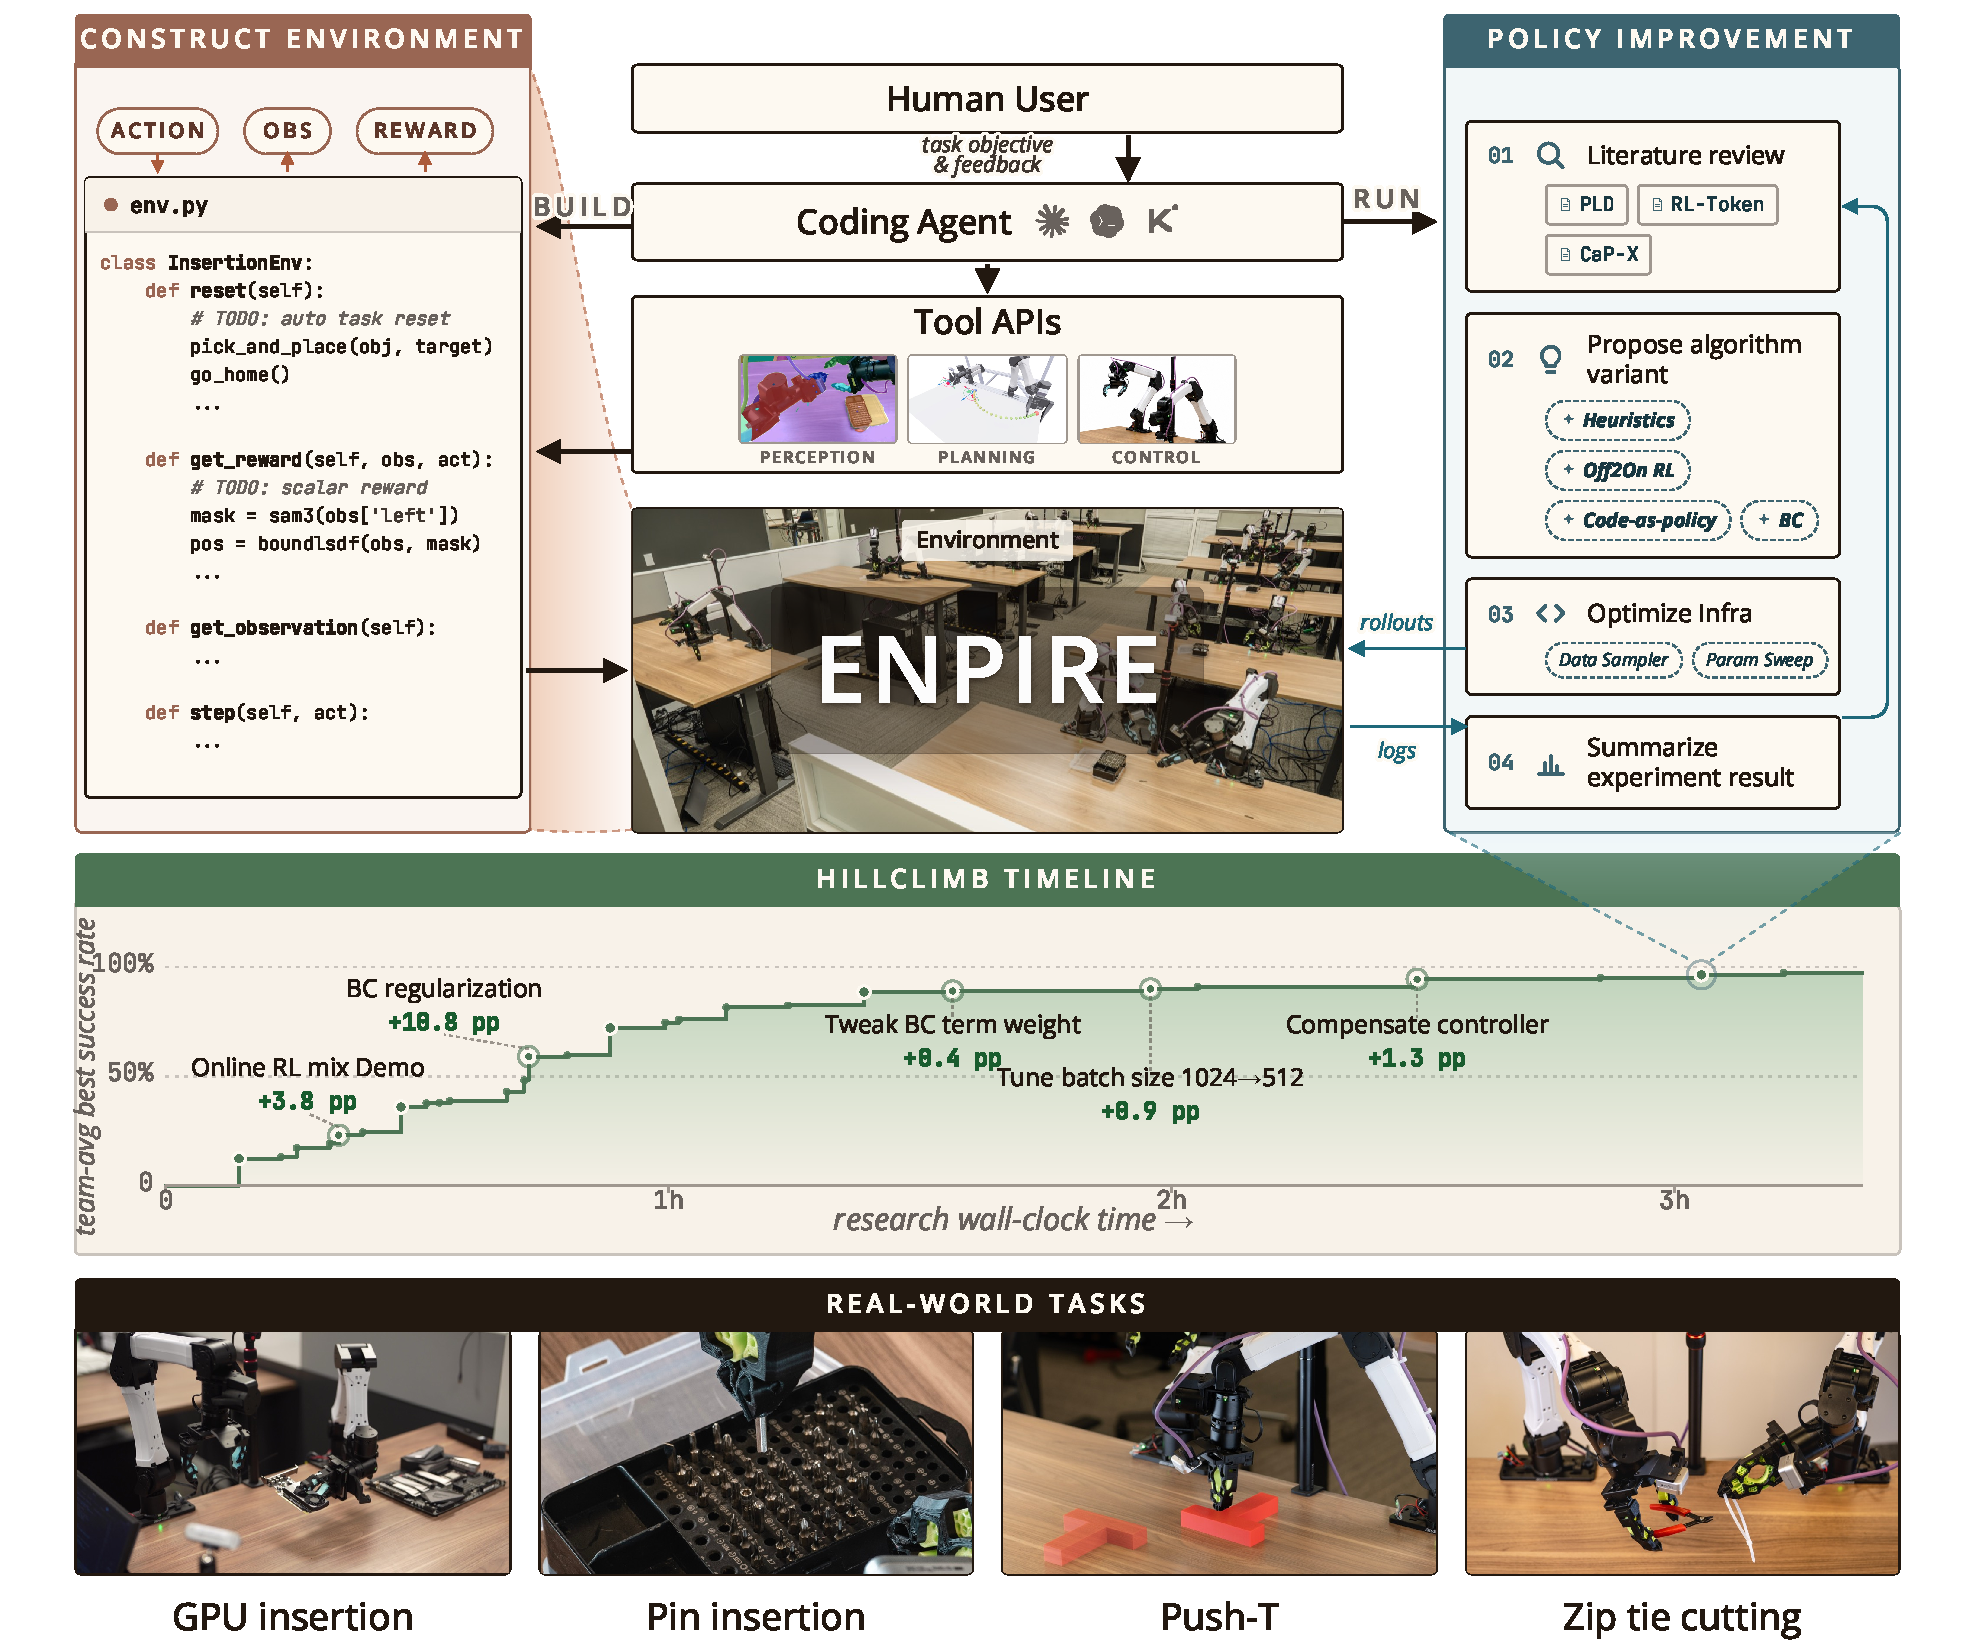
\includegraphics[width=1\linewidth,clip]{corl_2026_template_submission/figures/figure-v4.pdf}
    \caption{
    Overview of physical autoresearch framework \method. To solve a dexterous task in the real world, \method first uses tool calls to construct an environment with automatic reset and verification mechanisms according to human feedback. Next, the coding agent calls environment APIs to conduct autoresearch and hill-climb the policy success rate from real-world reward signals. More results are available at \website.
    % \textbf{1. Building environment module}. A coding agent iterates on an environment file under task objective and human feedback, calling perception, planning, and control tool APIs to close the observe–reward–act loop; the resulting \texttt{env.py} is packaged as the Environment. The shared components reused by both stages are the same coding agent, tool APIs, and environment. \textbf{2. Physical autoresearch}. The agent orchestrates a four-step loop — literature review, propose a variant, write training infra, summarize results — iterating round after round on top of that environment. \textbf{Hillclimb timeline}. Team-averaged best success rate (mean of the eight agents' personal bests) versus wall-clock time, rising in discrete cliffs; each Stage-2 round can lift the curve by one rung. \textbf{Real-world tasks}. The manipulation tasks studied — GPU insertion, pin insertion, Push-T, and zip-tie cutting.
    }
    \label{fig:overview}
\end{figure}


\section{Introduction}\label{sec:intro}
Automatically learning dexterous manipulation skills has been a major obstacle in the journey towards general physical intelligence. Frontier policy training methods, although highly effective, still rely on humans behind the scenes to participate in the data collection, evaluation with reset, and algorithm adjustment life cycle~\citep{pi05, recap, rl100}. As we scale up real-world policy learning,  humans labor of babysitting policy improvement inevitably become one of the limiting factors of how quickly robots acquire dexterity. 

Recent advances in autonomous research~\citep{karpathy2025autoresearch} (autoresearch), powered by coding agents, show a promising path toward automating algorithmic improvements. However, unique challenges arise when we extend this paradigm to automate real-world policy learning. First, coding agents lack a set of \emph{real-world environment interfaces} for closed-loop hypothesis testing in the physical world, which requires automated policy deployment, evaluation, and scene resetting. Second, when \emph{scaling up} autoresearch throughput across robot fleet, it remains an open problem to select and verify hypotheses while maintaining efficiency of resource utilization. 

To address these challenges, we introduce \method, an agent harness framework that leverages a suite of autonomous environment interfaces to enable scalable physical autoresearch. \method decomposes the acquisition of dexterous manipulation skills into two autoresearch procedures. In the first phase (\textbf{\texttt{{EN}}} in \method), coding agents construct an autonomous environment interface from human feedback. Through this initial research loop, agents implement and optimize procedural tool calls that establish safety boundaries, automated reset, and verification procedures for a specific task. They are optimized offline with a one-time setup cost; once finalized, they serve as immutable APIs that are reused throughout the subsequent stage. The second phase (\textbf{\texttt{{PIRE}}} in \method) transitions to a fully autonomous autoresearch procedure, where coding agents refine policies based on real-world feedback. Guided entirely by the environment's automated verification signals, the agents independently explore and optimize diverse methodologies to maximize real-world task success rates without human intervention. 

To scale this pipeline across multiple robots in parallel, \method introduces a mechanism to evolutionarily select hypotheses, which accelerates policy improvement. We dispatch a decentralized team of agents to test training recipes asynchronously, sharing and abandoning ideas based on the average success rates. The accumulated knowledge can be transferred to similar, novel tasks. 

\noindent We highlight the contributions of this work as follows:
\begin{itemize}[leftmargin=*, topsep=2pt, itemsep=2pt, parsep=0pt, partopsep=0pt]
  \item We formalize physical autoresearch for dexterous manipulation as a distinct problem for the coding agent and robotics communities. We propose to tackle this with a two-step approach: first, conducting a human-guided autoresearch to construct automatic environment feedback and verify it offline, then executing a fully autonomous autoresearch from real-world feedback in an online fashion to improve the policy. 
  \item We implement \method, an agentic harness through which a coding agent develops reusable robotic tools, constructs rewards and reset mechanisms with procedural tool calls, and effectively optimizes learning algorithms on real robots without human intervention. 
  \item We demonstrate that \method can hill-climb the success rate to a high level in multiple dexterous manipulation tasks. In pin insertion, policy convergence to 100\% is achieved faster than a frontier human-in-the-loop method~\citep{pld}. We also observe initial scaling behavior for parallelized autoresearch on a robot fleet and propose key metrics, Mean Token Utilization (MTU) and Mean Robot Utilization (MRU), to benchmark the efficiency of this procedure. 
\end{itemize}





% ablation: codex + opus, claude code: gpt, 
% Does the agent natively getting images
% use same harness, different model
% multiagent: open problem, potential other ways
% native multimodal vs multimodal as tool? let agent figure out [inspect whether native mm is enabled]
% turn on/off native multimodal capability
% take a dev log from previous dev log, [knowhow.md]

% \begin{tcolorbox}
% \red{
% Tonghe: revised introduction outline:\\
% 1. Automatically acquiring dexterity without human babysitting is a bottleneck\\
% 2. Autoresearch is an emerging automation method, working in the digital world, but why not for the physical world? \\
%     a. Why must you directly address the real? cannot solve with sim2real. Physics is hard to eliminate the gap from the sim design, and physical gym design is unavoidable. But maybe easier to simulate first in Sim as in Genesis. E.g., control bugs. latency. stochastic. Even you have those simple interfaces in simulation the sim2real physical grounding gap prevents faithfal mirroring in real performance (latency, friction changes, ..). Also real-world safety consequence. 
%     b. Why robotics-specific harness (and human collaboration needed: physical commonsense and safety to LLM agents. We have the access to robot/sensor device interfaces, but not abstraction level too low so not \emph{agent operatable}. Current LLM agents also lack robotics domain knowledge. Interfaces and human collaboration give llm agents physical commonsense (geometry, like what is left right top down topdown orientation pose) and grounding. 
%     c. Bottleneck to Scalability (iteration speed and feedback signal bottlenecked by realworld robot number)
%         * Scaling with operating time: Manual reset and reward automatic. This should be formulated as a subproblem of physical autoresearch to directly tackle prior to real world learning. 
%         * Scaling with robot number parallel verification. manage robot utility and token cost. Realworld robotics budget management, scaling in the future, consider the idle time. (automatic verification and reset and safety). Cannot easity parallelize to thousands of envs so requires low idle time per thread. Need speed per iter. And optimize for its speed. And also scalable to multiple tasks. 
%     d. Versatality need. Why more way more flexible than hyperparameter llm autoresearch, need ideation level research. paradigm agnostic, because robot learning research have not converged yet like language models.  So we support various kinds of learning paradigms. 
% 3. Env construction needs manual labor. Can we resue those stuffs, and offline get it fast and correct? one-time cost. \\
% * Env construciton itself is a research problem that has to be automated to reuse this in the future (fixed investment)\\
% * Physical autoresearch and its difference from LLM autoresearch:   \\
% 0. Formalize the physical autoresearch problem in real world policy learning. 
% 1. real robot hardware, real-time. \\
% 2. ideation level research (paradigm not converged yet): not just hyperparam sweep. beyond learning paradigm (beyond hyperpam search as the original). Because robotics paradigm have not converged yet\\
% 3. agent teams and robot fleet. should simultaneously optimize token and robot utility as it is an important part of phys autoresearch \\
% * Limitation: in the future, leverage the sim to speed up real eval design, cite genesis. 
% * Stop talking about skill library in main paper. Just say collaborate with humans based on basic perception /control APIs. 
% }
% \end{tcolorbox}


% \guanzhi{The narrative flow feels slightly unnatural here. After introducing the gap without actually explaining it, the paper immediately introduces the setup/problem formulation before explaining why physical auto-research is fundamentally difficult. I think the challenge/asymmetry discussion (physical grounding, budget limitation, no pre-built environment) could come earlier.}

% \guanzhi{I feel the deeper distinction is not whether the environment exists, but whether it is already agent-operable. Digital environments are typically programmatically accessible by agents by default (evaluation, metrics, resets, supervision), whereas physical robotics exposes raw embodiment but not the operational interfaces required for autonomous experimentation.}

% \guanzhi{Shall we frame this around “offline-verifiable components” instead? “atomic-snippet workflow” sounds more implementation-specific.}
% \guanzhi{robotics toolkit sounds too generic. What's different from the CaP-X-style toolkit?}
% \guanzhi{Do we want to mention agent teams here?}
% \guanzhi{This paragraph feels disconnected because it introduces the core conceptual thesis only after the method/design choices have already been presented. Maybe move this earlier before introducing the method.}


















% \begin{figure}
%     \centering
%     \includegraphics[width=0.5\linewidth]{mru_mtu.png}
%     \caption{MRU and MTU}
%     \label{fig:mru_mtu}
% \end{figure}






















% This paper is a positioning contribution. \method is not optimal; it is a first viable system for what we believe is a fundamental problem at the intersection of LLM-based agents and robotics. The design space we explore is non-exhaustive, and end-to-end performance is bounded by the perception and tool-use capabilities of the underlying agent. To enable follow-up work, we release a physical auto-research benchmark together with a simulated counterpart, so that the LLM-agent and robotics communities can reproduce, compete with, and surpass our results without requiring bimanual hardware.






% Automating robotics research on physical hardware is a defining challenge for embodied AI. Real-world experiments require a great amount of human labor to set up the evaluation environment and babysit the robot, limiting the efficiency of iterating on new ideas. In the digital domain, recent progress in coding agents powered by large language models has begun to automate labor by iteratively proposing, implementing, evaluating, and refining code; they reach substantial autonomy in software engineering \citep{jimenez2024swebench, yang2024swe}, machine-learning research \citep{lu2024aiscientist, yamada2025aiscientistv2, karpathy2025autoresearch}, digital embodied environments \citep{wang2023voyager, ma2024eureka}. Despite coding agents demonstrating capabilities of operating in the physical world, e.g., synthesis of executable robot policies from natural-language goals \citep{liang2023cap, capx2026} and collecting real-world data at scale \citep{ahn2024autort}, there still exists a non-trivial gap to harness the coding agent for autonomously improving policy or algorithms measured by real-world performance. (TODO: Add more contextual description of the gap) 


% In this paper, we study whether it is possible to enable the state-of-the-art coding agents (cite Claude \& Codex) to achieve \emph{autonomous policy improvement on real robot hardware}. Given a manipulation task and context (including textual description, human demonstration, or base policy checkpoint), the agent is challenged to deliver a high-performance policy, assuming access to a real robot hardware and a basic toolkit for vision and control. The agent can either develop reusable code primitives and output code-as-policy \citep{liang2023cap, capx2026},
% or study algorithmic choices to train an end-to-end policy either online or offline. This challenge is set apart from its digital counterparts \citep{jimenez2024swebench} by: 
% (1) \emph{Physical grounding} Assumptions need to be verified by evaluation on real hardware, and performance only assessed upon deployment.
% (2) \emph{Budget limitation}  Digital candidates parallelize across commodity hardware and scale with money: a thousand architectures can be trained on ImageNet by buying a thousand GPUs. Physical experiments occupy a few robots per trial, run serially in wall-clock time, and deplete a hardware-time budget that computation cannot grow.
% (3) \emph{No pre-built environment.} Digital environments are typically programmatically accessible by agents by default. However, physical robots expose raw interfaces for control and sensing, which are not trivially agent-operable.


% To address this challenge, we introduce \method, an agent-harness framework for autonomous policy improvement on real robot hardware. Given a manipulation problem and a finite budget of robot access time, \method orchestrates a self-improvement loop in which the agent constructs experimental environments, including resets and verifiable rewards. Then, it would develop reusable robotics tools and schedule experiments within the robot budget. 
% \method derives its autonomy from three design choices (Fig.~\ref{fig:pipeline}). \emph{(i) An atomic-snippet workflow.} The agent is required to author and unit-test individual skills, rewards, and reset routines in isolation before composition, applying self-verification and skill-synthesis principles \citep{shinn2023reflexion, wang2023voyager} to the physical regime.  \emph{(ii) A shared robotics toolkit.} Reusable perception and manipulation modules---vision-language models, segmentation, motion planning, and grasping---are exposed as callable primitives that the agent composes into both experimental environments and candidate policies, extending the code-as-policy paradigm \citep{liang2023codeaspolicies, capx2026} from policy synthesis to the construction of the full research loop.  \emph{(iii) Persistent experiment logging and memory.} Execution traces, intermediate artifacts, and verified components are recorded across iterations, allowing the agent to recover from failures and to reuse prior work rather than revalidate it from scratch.

% % takeaway and results

% Our central idea is that this asymmetry is exploitable, not insurmountable. Most determinants of a research step's success in physical robotics---whether a detector localizes the right object, whether a reward returns sensible values on cached sensor logs, whether a reset is collision-free in motion-planner simulation---can be evaluated without consuming the experiment budget. The agent's job is therefore to validate components of the robot, where verification is cheap, and to commit hardware time only when a decision genuinely requires physical interaction. We accordingly take the unit of autonomous progress to be the offline-verifiable component (perception module, reward function, reset routine, controller), not the end-to-end trial; constructing a Gym-style environment on bare hardware is itself the agent's first research action, not a precondition supplied to it. The three design choices in \method are direct consequences of this idea: the atomic-snippet workflow operationalizes off-robot component verification, the toolkit gives the agent the primitives to author environments and policies in code, and persistent memory amortizes the cost of each verified component across the research loop.

% %To make physical auto-research systems measurable and comparable, we introduce two resource-utilization metrics: \textbf{Mean Robot Usage (MRU)}, the fraction of allocated robot-access time the system spends executing experiments rather than idling, recompiling, or recovering from faults; and \textbf{Mean FLOPs Utility (MFU)}, the analogous metric for compute. We treat MRU and MFU as utilization axes complementary to task-level outcomes such as final success rate and improvement per unit budget; together they characterize how efficiently a scarce physical resource is converted into research progress.

% Deployed on a YAM bimanual manipulator across four contact-rich and dexterous tasks spanning learning paradigms, \method achieves consistent hill-climbing of task performance under a fixed robot budget. (TODO, more results)
% %On pin insertion, the agent autonomously selected a non-learning solution path: rather than training a neural policy, it determined that a rule-based controller composed of its own toolkit was sufficient, and reached 100\% success within 1.5 hours of robot access -- faster than direct SAC training under matched conditions \citep{xiao2025self}. Using the same protocol, we further benchmark recent frontier coding agents (Claude Opus~4.7, CodeX) on this suite, and observe initial scaling behavior when \method is deployed in parallel across multiple robots.


\ifdefined\nvidiareleaseomitsharedteaser
\else
\begin{figure}
    \centering
    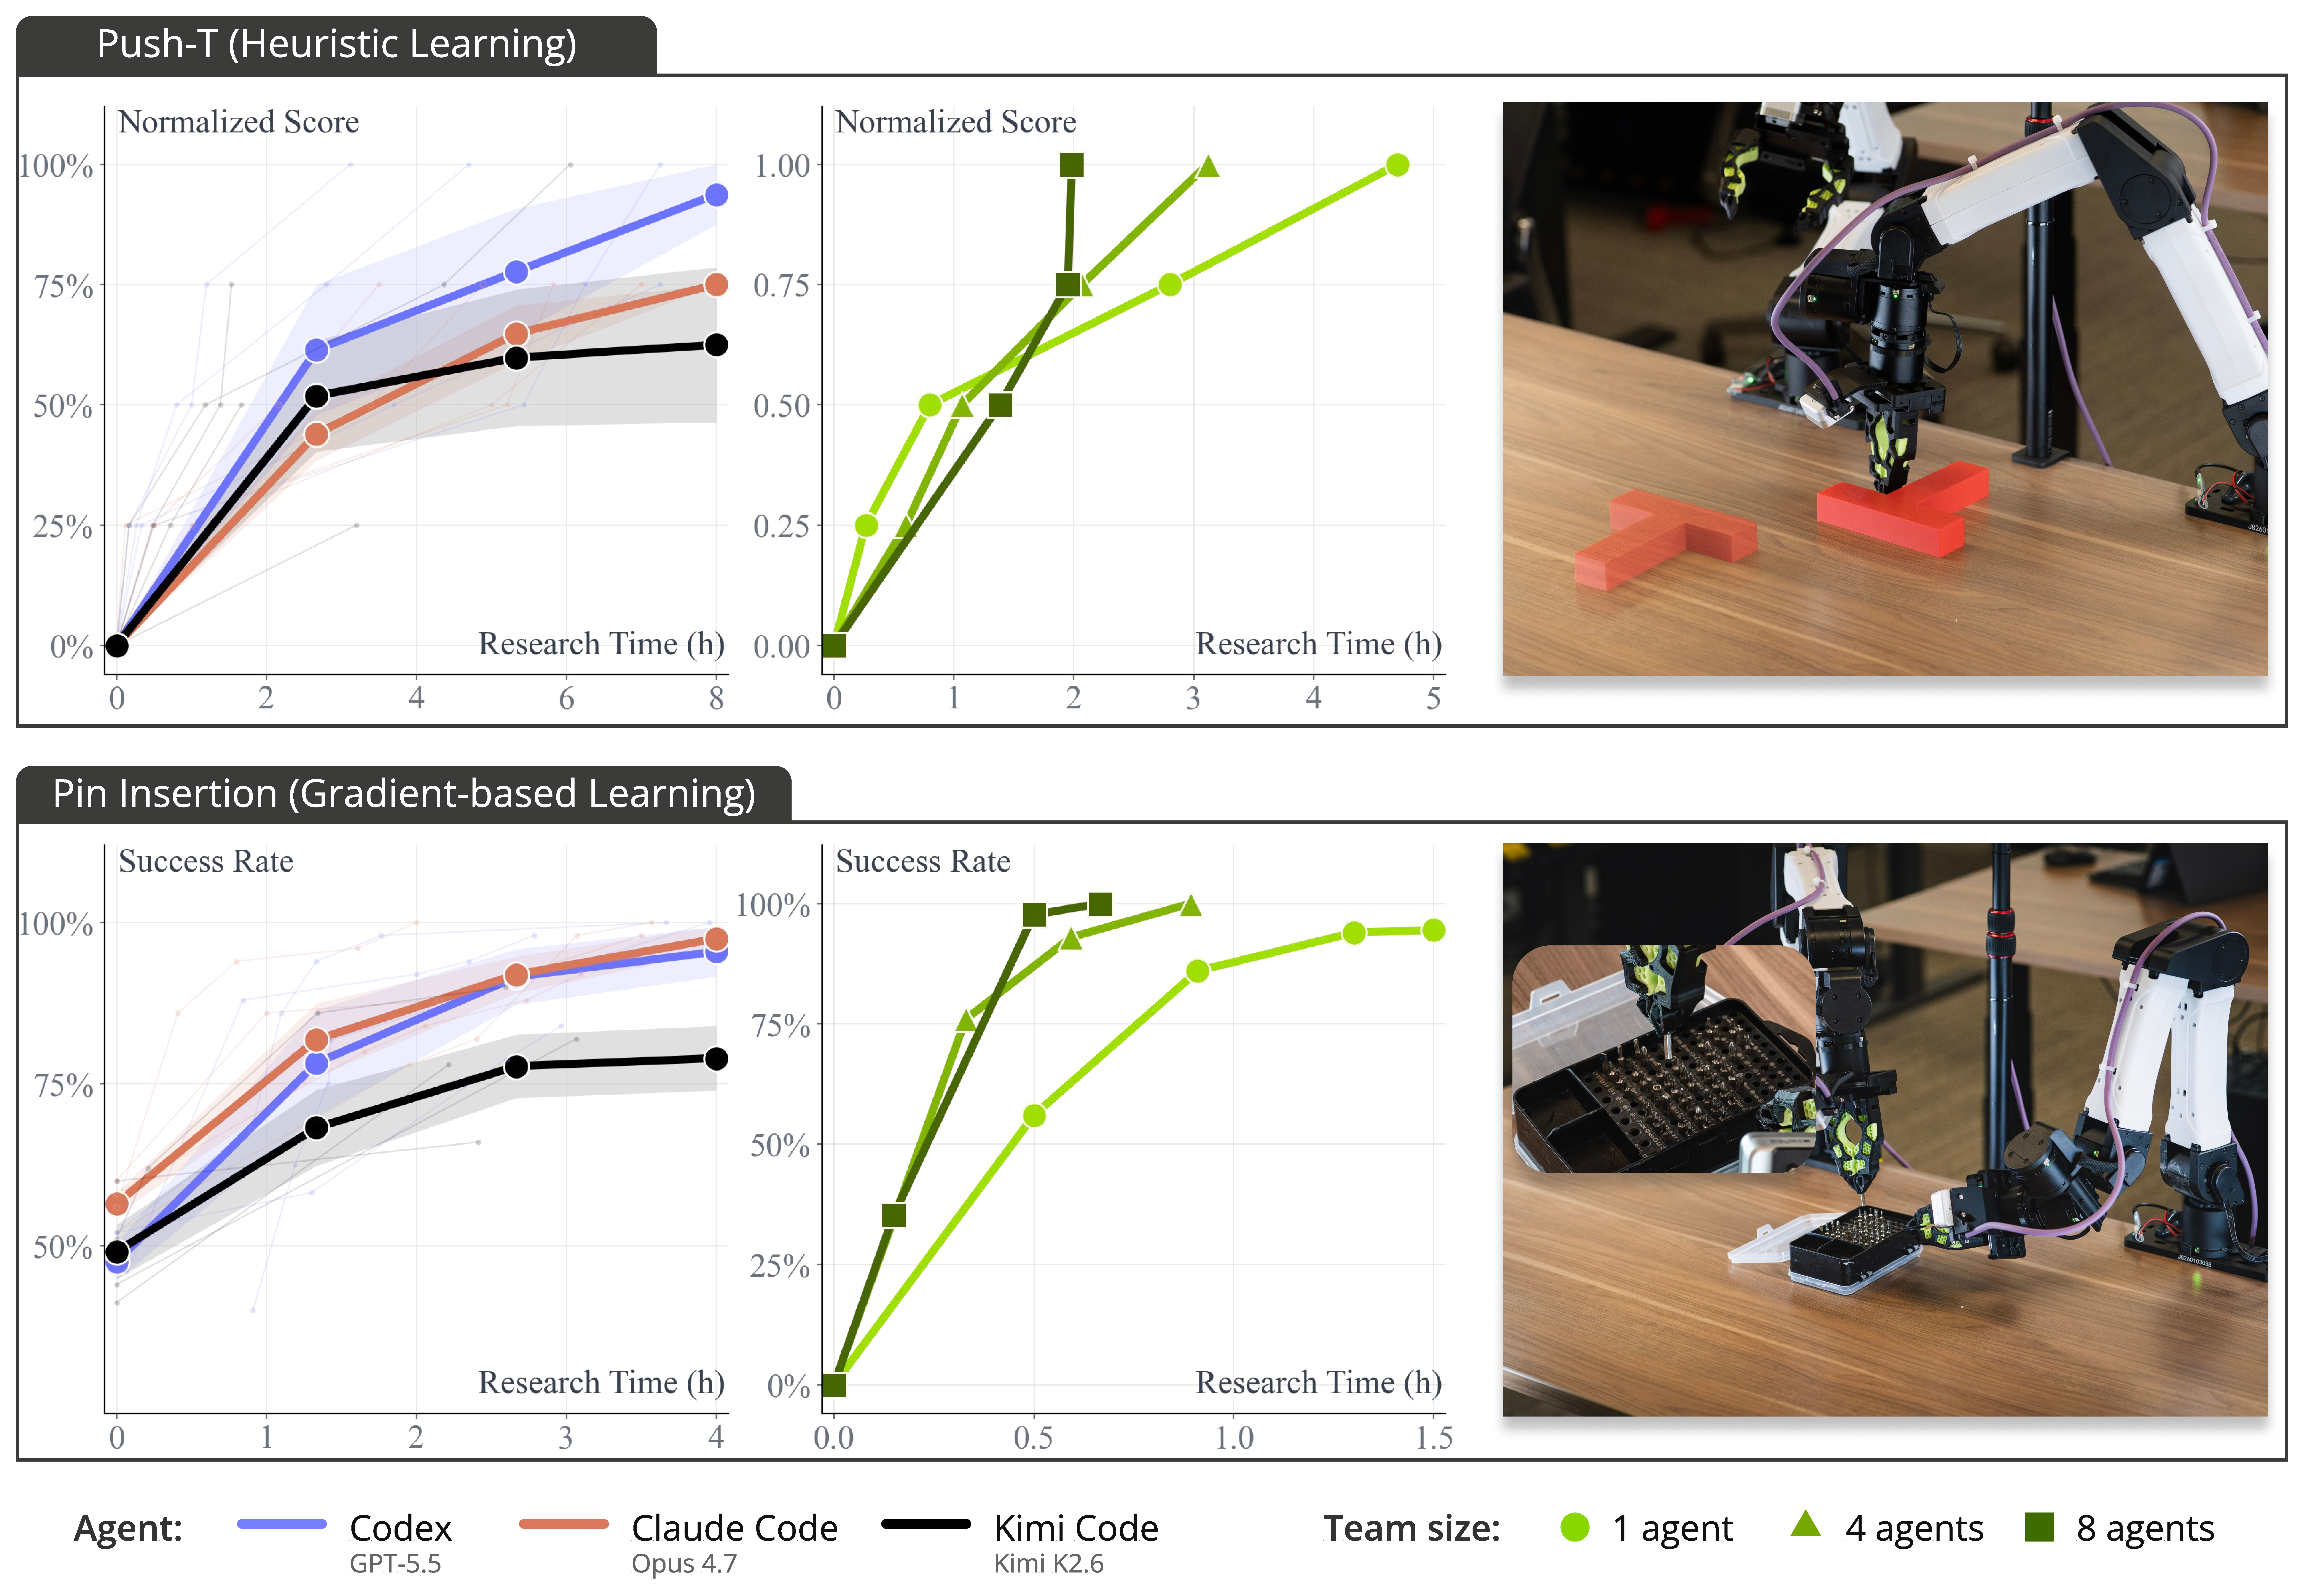
\includegraphics[width=0.8\linewidth]{corl_2026_template_submission/figures/auto_env_bench.pdf}
    \caption{\textbf{Benchmarking coding agents for physical autoresearch}. \method enables \texttt{state-of-the-art} coding agents to achieve autonomous policy improvement on \textbf{Push-T} and \textbf{Pin Insertion} tasks. \method also scales with resources, as increasing the number of robot agent workers reduces the wall-clock time required to reach the same task performance.} 
    \label{fig:real_pusht_pin_insertion}
\end{figure}
\fi
